\documentclass{standalone}
\usepackage{tikz}
\usetikzlibrary{patterns, positioning}


\begin{document}
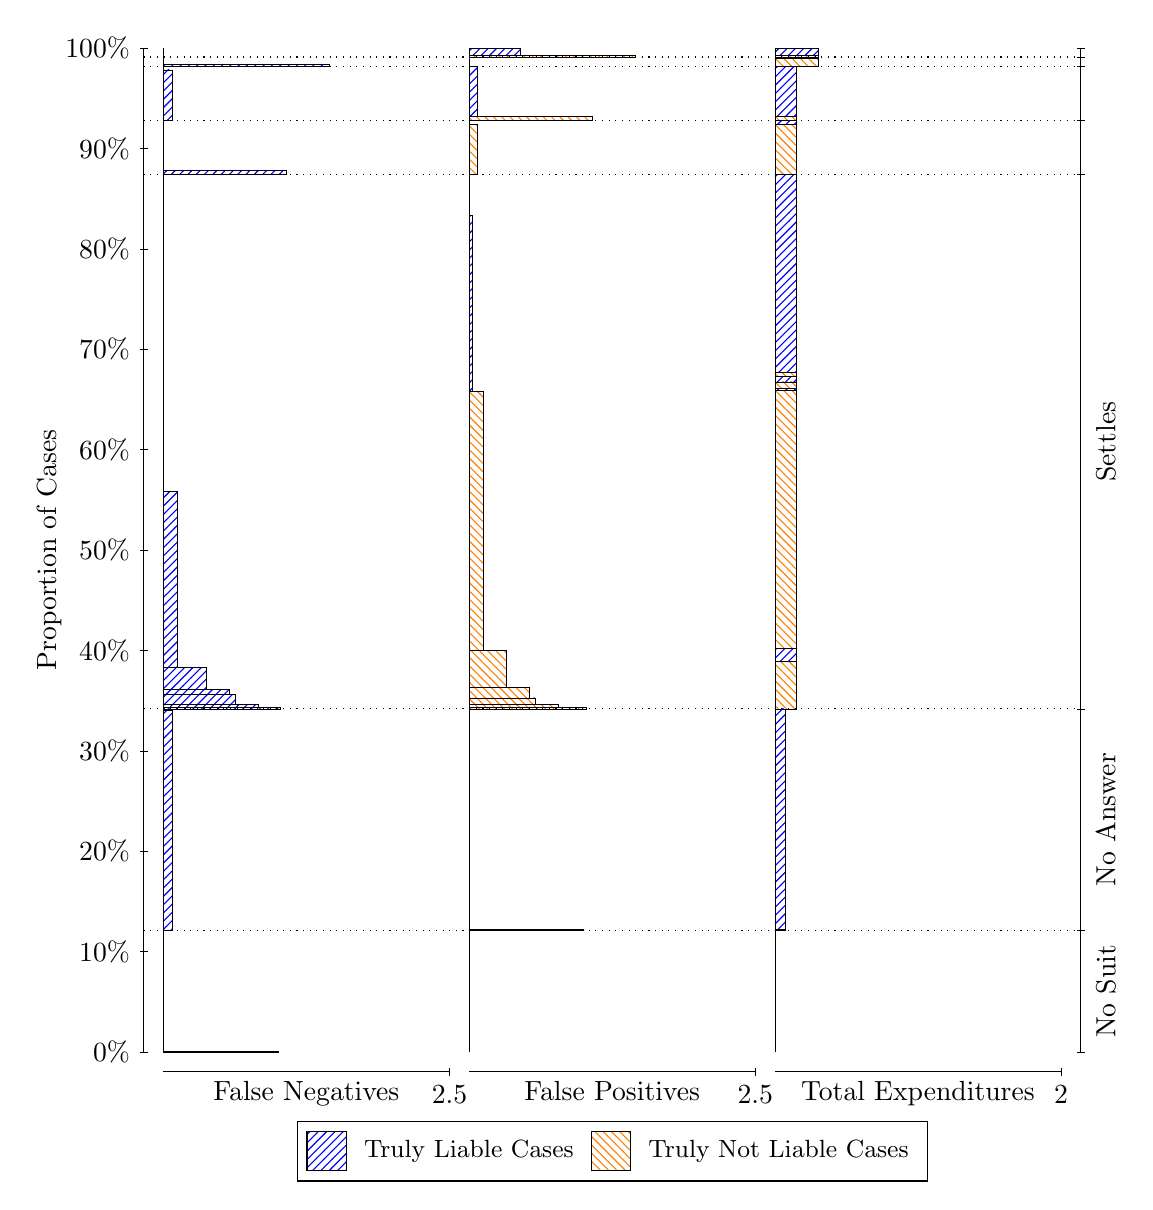
\begin{tikzpicture}
\draw[black, very thin] (1.5,1.75) -- (1.5,14.5);
\node[rotate=90, text=black, anchor=center] at (0.3, 8.125) {Proportion of Cases};
\draw[black, very thin] (1.45,1.75) -- (1.55,1.75);
\node[text=black, anchor=east] at (1.45, 1.75) {0\%};
\draw[black, very thin] (1.45,3.025) -- (1.55,3.025);
\node[text=black, anchor=east] at (1.45, 3.025) {10\%};
\draw[black, very thin] (1.45,4.3) -- (1.55,4.3);
\node[text=black, anchor=east] at (1.45, 4.3) {20\%};
\draw[black, very thin] (1.45,5.575) -- (1.55,5.575);
\node[text=black, anchor=east] at (1.45, 5.575) {30\%};
\draw[black, very thin] (1.45,6.85) -- (1.55,6.85);
\node[text=black, anchor=east] at (1.45, 6.85) {40\%};
\draw[black, very thin] (1.45,8.125) -- (1.55,8.125);
\node[text=black, anchor=east] at (1.45, 8.125) {50\%};
\draw[black, very thin] (1.45,9.4) -- (1.55,9.4);
\node[text=black, anchor=east] at (1.45, 9.4) {60\%};
\draw[black, very thin] (1.45,10.675) -- (1.55,10.675);
\node[text=black, anchor=east] at (1.45, 10.675) {70\%};
\draw[black, very thin] (1.45,11.95) -- (1.55,11.95);
\node[text=black, anchor=east] at (1.45, 11.95) {80\%};
\draw[black, very thin] (1.45,13.225) -- (1.55,13.225);
\node[text=black, anchor=east] at (1.45, 13.225) {90\%};
\draw[black, very thin] (1.45,14.5) -- (1.55,14.5);
\node[text=black, anchor=east] at (1.45, 14.5) {100\%};

\draw[black, very thin] (13.4,1.75) -- (13.4,14.5);
\draw[black, very thin] (13.35,1.75) -- (13.45,1.75);
\node[anchor=west] at (13.35, 1.75) {};
\draw[black, very thin] (13.35,3.2907) -- (13.45,3.2907);
\node[anchor=west] at (13.35, 3.2907) {};
\draw[black, very thin] (13.35,6.108) -- (13.45,6.108);
\node[anchor=west] at (13.35, 6.108) {};
\draw[black, very thin] (13.35,12.894) -- (13.45,12.894);
\node[anchor=west] at (13.35, 12.894) {};
\draw[black, very thin] (13.35,13.583) -- (13.45,13.583);
\node[anchor=west] at (13.35, 13.583) {};
\draw[black, very thin] (13.35,14.271) -- (13.45,14.271);
\node[anchor=west] at (13.35, 14.271) {};
\draw[black, very thin] (13.35,14.386) -- (13.45,14.386);
\node[anchor=west] at (13.35, 14.386) {};
\draw[black, very thin] (13.35,14.5) -- (13.45,14.5);
\node[anchor=west] at (13.35, 14.5) {};

\draw[black, very thin, pattern color=blue, pattern=north east lines] (1.75,1.75) rectangle (3.2033,1.7539);
\draw[black, very thin, pattern color=orange, pattern=north west lines] (1.75,1.7539) rectangle (1.75,3.2907);
\draw[black, very thin, pattern color=blue, pattern=north east lines] (1.75,3.2907) rectangle (1.859,6.0943);
\draw[black, very thin, pattern color=orange, pattern=north west lines] (1.75,6.0943) rectangle (1.75,6.108);
\draw[black, very thin, pattern color=blue, pattern=north east lines] (1.75,6.108) rectangle (3.2397,6.1257);
\draw[black, very thin, pattern color=blue, pattern=north east lines] (1.75,6.1257) rectangle (2.949,6.1669);
\draw[black, very thin, pattern color=blue, pattern=north east lines] (1.75,6.1669) rectangle (2.6583,6.2871);
\draw[black, very thin, pattern color=blue, pattern=north east lines] (1.75,6.2871) rectangle (2.5857,6.3549);
\draw[black, very thin, pattern color=blue, pattern=north east lines] (1.75,6.3549) rectangle (2.295,6.6304);
\draw[black, very thin, pattern color=blue, pattern=north east lines] (1.75,6.6304) rectangle (1.9317,8.8674);
\draw[black, very thin, pattern color=orange, pattern=north west lines] (1.75,8.8674) rectangle (1.75,12.894);
\draw[black, very thin, pattern color=blue, pattern=north east lines] (1.75,12.894) rectangle (3.3123,12.949);
\draw[black, very thin, pattern color=orange, pattern=north west lines] (1.75,12.949) rectangle (1.75,13.583);
\draw[black, very thin, pattern color=blue, pattern=north east lines] (1.75,13.583) rectangle (1.859,14.222);
\draw[black, very thin, pattern color=orange, pattern=north west lines] (1.75,14.222) rectangle (1.75,14.271);
\draw[black, very thin, pattern color=blue, pattern=north east lines] (1.75,14.271) rectangle (3.8573,14.289);
\draw[black, very thin, pattern color=orange, pattern=north west lines] (1.75,14.289) rectangle (1.75,14.386);
\draw[black, very thin, pattern color=orange, pattern=north west lines] (1.75,14.386) rectangle (1.75,14.403);
\draw[black, very thin, pattern color=blue, pattern=north east lines] (1.75,14.403) rectangle (1.75,14.5);
\draw[black, very thin, pattern color=orange, pattern=north west lines] (5.6333,1.75) rectangle (5.6333,3.2868);
\draw[black, very thin, pattern color=blue, pattern=north east lines] (5.6333,3.2868) rectangle (5.6333,3.2907);
\draw[black, very thin, pattern color=orange, pattern=north west lines] (5.6333,3.2907) rectangle (7.0867,3.3044);
\draw[black, very thin, pattern color=blue, pattern=north east lines] (5.6333,3.3044) rectangle (5.6333,6.108);
\draw[black, very thin, pattern color=orange, pattern=north west lines] (5.6333,6.108) rectangle (7.123,6.1281);
\draw[black, very thin, pattern color=orange, pattern=north west lines] (5.6333,6.1281) rectangle (6.7597,6.162);
\draw[black, very thin, pattern color=orange, pattern=north west lines] (5.6333,6.162) rectangle (6.469,6.2476);
\draw[black, very thin, pattern color=orange, pattern=north west lines] (5.6333,6.2476) rectangle (6.3963,6.3782);
\draw[black, very thin, pattern color=orange, pattern=north west lines] (5.6333,6.3782) rectangle (6.1057,6.8539);
\draw[black, very thin, pattern color=orange, pattern=north west lines] (5.6333,6.8539) rectangle (5.815,10.135);
\draw[black, very thin, pattern color=blue, pattern=north east lines] (5.6333,10.135) rectangle (5.6697,12.372);
\draw[black, very thin, pattern color=blue, pattern=north east lines] (5.6333,12.372) rectangle (5.6333,12.894);
\draw[black, very thin, pattern color=orange, pattern=north west lines] (5.6333,12.894) rectangle (5.7423,13.528);
\draw[black, very thin, pattern color=blue, pattern=north east lines] (5.6333,13.528) rectangle (5.6333,13.583);
\draw[black, very thin, pattern color=orange, pattern=north west lines] (5.6333,13.583) rectangle (7.1957,13.632);
\draw[black, very thin, pattern color=blue, pattern=north east lines] (5.6333,13.632) rectangle (5.7423,14.271);
\draw[black, very thin, pattern color=orange, pattern=north west lines] (5.6333,14.271) rectangle (5.6333,14.368);
\draw[black, very thin, pattern color=blue, pattern=north east lines] (5.6333,14.368) rectangle (5.6333,14.386);
\draw[black, very thin, pattern color=orange, pattern=north west lines] (5.6333,14.386) rectangle (7.7407,14.403);
\draw[black, very thin, pattern color=blue, pattern=north east lines] (5.6333,14.403) rectangle (6.2873,14.5);
\draw[black, very thin, pattern color=orange, pattern=north west lines] (9.5167,1.75) rectangle (9.5167,3.2868);
\draw[black, very thin, pattern color=blue, pattern=north east lines] (9.5167,3.2868) rectangle (9.5167,3.2907);
\draw[black, very thin, pattern color=orange, pattern=north west lines] (9.5167,3.2907) rectangle (9.6529,3.3044);
\draw[black, very thin, pattern color=blue, pattern=north east lines] (9.5167,3.3044) rectangle (9.6529,6.108);
\draw[black, very thin, pattern color=orange, pattern=north west lines] (9.5167,6.108) rectangle (9.7892,6.7143);
\draw[black, very thin, pattern color=blue, pattern=north east lines] (9.5167,6.7143) rectangle (9.7892,6.8757);
\draw[black, very thin, pattern color=orange, pattern=north west lines] (9.5167,6.8757) rectangle (9.7892,10.156);
\draw[black, very thin, pattern color=blue, pattern=north east lines] (9.5167,10.156) rectangle (9.7892,10.174);
\draw[black, very thin, pattern color=orange, pattern=north west lines] (9.5167,10.174) rectangle (9.7892,10.26);
\draw[black, very thin, pattern color=blue, pattern=north east lines] (9.5167,10.26) rectangle (9.7892,10.328);
\draw[black, very thin, pattern color=orange, pattern=north west lines] (9.5167,10.328) rectangle (9.7892,10.381);
\draw[black, very thin, pattern color=blue, pattern=north east lines] (9.5167,10.381) rectangle (9.7892,12.894);
\draw[black, very thin, pattern color=orange, pattern=north west lines] (9.5167,12.894) rectangle (9.7892,13.528);
\draw[black, very thin, pattern color=blue, pattern=north east lines] (9.5167,13.528) rectangle (9.7892,13.583);
\draw[black, very thin, pattern color=orange, pattern=north west lines] (9.5167,13.583) rectangle (9.7892,13.632);
\draw[black, very thin, pattern color=blue, pattern=north east lines] (9.5167,13.632) rectangle (9.7892,14.271);
\draw[black, very thin, pattern color=orange, pattern=north west lines] (9.5167,14.271) rectangle (10.062,14.368);
\draw[black, very thin, pattern color=blue, pattern=north east lines] (9.5167,14.368) rectangle (10.062,14.386);
\draw[black, very thin, pattern color=orange, pattern=north west lines] (9.5167,14.386) rectangle (10.062,14.403);
\draw[black, very thin, pattern color=blue, pattern=north east lines] (9.5167,14.403) rectangle (10.062,14.5);
\draw[black, dotted] (1.5,3.2907) -- (13.4,3.2907);
\draw[black, dotted] (1.5,6.108) -- (13.4,6.108);
\draw[black, dotted] (1.5,12.894) -- (13.4,12.894);
\draw[black, dotted] (1.5,13.583) -- (13.4,13.583);
\draw[black, dotted] (1.5,14.271) -- (13.4,14.271);
\draw[black, dotted] (1.5,14.386) -- (13.4,14.386);
\draw[black, very thin] (1.75,1.5) -- (5.3833,1.5);
\node[text=black, anchor=north] at (3.5667, 1.5) {False Negatives};
\draw[black, very thin] (5.3833,1.45) -- (5.3833,1.55);
\node[text=black, anchor=north] at (5.3833, 1.45) {2.5};

\draw[black, very thin] (5.6333,1.5) -- (9.2667,1.5);
\node[text=black, anchor=north] at (7.45, 1.5) {False Positives};
\draw[black, very thin] (9.2667,1.45) -- (9.2667,1.55);
\node[text=black, anchor=north] at (9.2667, 1.45) {2.5};

\draw[black, very thin] (9.5167,1.5) -- (13.15,1.5);
\node[text=black, anchor=north] at (11.333, 1.5) {Total Expenditures};
\draw[black, very thin] (13.15,1.45) -- (13.15,1.55);
\node[text=black, anchor=north] at (13.15, 1.45) {2};

\node[text=black, centered, rotate=90] at (13.72, 2.5204) {No Suit};
\node[text=black, centered, rotate=90] at (13.72, 4.6994) {No Answer};
\node[text=black, centered, rotate=90] at (13.72, 9.501) {Settles};





\draw (7.449999999999999,1.5) node[draw=none] (baseCoordinate) {};
\begin{scope}[align=center]
        \matrix[scale=0.5, draw=black, below=0.5cm of baseCoordinate, nodes={draw}, column sep=0.1cm]{
            \node[rectangle, draw, minimum width=0.5cm, minimum height=0.5cm, pattern color=blue, pattern=north east lines] {}; &
            \node[draw=none, font=\small, text=black] (B) {Truly Liable Cases}; &
            \node[rectangle, draw, minimum width=0.5cm, minimum height=0.5cm, pattern color=orange, pattern=north west lines] {}; &
            \node[draw=none, font=\small, text=black] (B) {Truly Not Liable Cases}; \\
            };
\end{scope}

\end{tikzpicture}
\end{document}